\documentclass{beamer}

% select theme
\usetheme{CambridgeUS}
\usecolortheme{beaver}

\usepackage{kotex}
\usepackage{fancyvrb}
\usepackage{color}
\usepackage[mmddyyyy]{datetime}
\usepackage{pythontex}
\usepackage{graphicx, subfigure}

% you need to generate pyg.tex by
% pygmentize -O full -f latex hello.c
% \input{pyg.tex}



% syntax highlighted source code 넣는법:
% http://ubuntuforums.org/showthread.php?t=790610
% pygmentize 명령어가 실행될 수 있도록 하자.
% bash에 그냥 pygmentize라고 치면 어느 패키지를 설치해야 하는지 알려줌.
% then...
% 색깔 명령어가 define될 수 있도록... hello.c를 만든 다음,
% pygmentize -O full -f latex hello.c
% 를 돌리면 무엇을 include해야 하는지, define이 뭐가 필요한지 쭉
% stdout으로 출력해줌.
% pygmentize -f latex hello.c 로 나오는 verbatim문을 긁어붙이면 완성.
\begin{document}

% title slide
\begin{frame}
	\title{Decision Making}
	\author{정민우}
	\date{\today}
	\titlepage
\end{frame}

% outline slide
\section*{Outline}
\begin{frame}
\tableofcontents
\end{frame}

\section{Markov Process}
\begin{frame}
	미리 정의된 어떤 확률 분포를 따라 상태와 상태 사이를 이동해 다니는 여정\\
	메모리를 갖지 않는 이산 시간 확률 과정\\
	확률과정\\
	시간의 흐름에 따라 상태가 확률적으로 변화하는 과정\\
	확률 분포를 따르는 임의변수(random variable)가 discrete한 time interval마다 값을 생성하는 것\\
	현재 상태(state)가 이전 상태에만 영향을 받는 확률 과정\\
	미래는 오로지 현재에 의해 결정됨\\
	상태가 변화하는 과정은 확률 계산에 영향을 미치지 않음\\
	단일 상태 정보만으로 정보가 충분하도록 상태를 잘 구성해야 함\\
	
	\begin{figure}
		\subfigure{\includegraphics[width=0.3\columnwidth]{Fig/Markov Chain Example.pdf}}
		% \hspace{0.8cm}
		% \subfigure{\includegraphics[width=0.3\columnwidth]{../Figure/Figure_14.pdf}}
		% \subfigure{\includegraphics[width=0.4\columnwidth]{../Figure/Figure_15.pdf}}
	\end{figure}
\end{frame}

\begin{frame}
	\frametitle{Markov Property}
		어떤 시간에 특정 상태에 도달하든 그 이전에 어떤 상태를 거쳐왔든 다음 상태로 갈 확률은 항상 같음\\
		미래는 과거와 독립적인 것\\
		Memoryless property\\
		\begin{equation}\label{markov property}
			Pr(S_{t+1} = s' | S_0, S_1, ..., S_{t-1}, S_t) = Pr(S_{t+1} = s' | S_t)
		\end{equation}
		Terminal state\\
		Stationary distribution\\
\end{frame}

\begin{frame}
	\frametitle{State Transition Probability Matrix}
		Transition : state 간 이동\\
		State transition probability : 확률적 transition\\
		\begin{equation}\label{state transition probability}
			P_{ss'} = Pr(S_{t+1} = s' | S_t = s)
		\end{equation}
		Transition probability를 행렬 형태로 정리한 것\\
\end{frame}

\section{Markov Reward Process(MRP)}
\begin{frame}
	\frametitle{Reward}
		Markov process에 reward 개념을 추가하는 것\\
		Reward는 transition에 대한 가중치를 추가하는 것\\
		\begin{equation}\label{immediate reward}
			R_s = E[r_{t+1} | S_t = s]
		\end{equation}
\end{frame}

\begin{frame}
	\frametitle{Discounting factor}
		감가율\\
		현재와 미래의 가치 차이가 발생함\\		
\end{frame}

\begin{frame}
	\frametitle{Return}
		미래에 얻을 수 있는 total reward 예측 가능함\\
		각 시점에서 immediate reward들을 현재가치로 환산하여 합한 값\\
		\begin{equation}\label{return}
			G_t = R_{t+1}+R_{t+2}+... = \sum^\infty_{k=0}(\gamma^kR_{t+k+1})
		\end{equation}		
\end{frame}

\begin{frame}
	\frametitle{Value Function of MRP}
		state의 가치를 표현하는 함수\\
		특정 state에서 미래에 얻을 수 있는 모든 reward를 더한 것에 대한 expectation\\
		state에서 이동 가능한 state들의 시나리오들을 따라 reward에 discounting factor를 적용하여 합한 값\\
		\begin{equation}\label{value function}
			V(s) = E[G_{t} | S_{t} = s]
		\end{equation}		
\end{frame}

\section{Markov Decision Process}
어떤 문제를 컴퓨터로 풀기 위해서 수학적으로 정의되어야 함\\
Markov decision process는 의사결정 과정을 모델링하는 틀을 제공함\\

\begin{frame}
	\frametitle{Action}
		MRP에 agent 개념이 추가됨\\	
		Agent는 각 상황마다 Action\\
		\begin{equation}\label{MDP}
			MDP \equiv (S, A, P, R, \gamma)
		\end{equation}
		S : 상태집합\\
		A : 액션집합\\
		P : 전이확률행\\
		R : 보상함수\\
		gamma : 감쇠인자\\
\end{frame}

\begin{frame}
	\frametitle{Policy}
		state에서 action을 mapping하는 함수\\	
		해당 state에서 어떤 action을 할 지 정하는 것\\
		\begin{equation}\label{policy}
			\phi(a|s) = Pr(A_{t} = a | S_{t} = s)
		\end{equation}
		강화학습의 목적은 return을 최대화 할 수 있는 policy를 찾는 것\\
		Return을 최대화하는 action을 선택하는 함수를 찾는 것\\
\end{frame}

\begin{frame}
	\frametitle{Value Function of MDP}
		\begin{figure}
			\subfigure{\includegraphics[width=0.4\columnwidth]{Fig/MDP.pdf}}
		\end{figure}		
		t 시점에 state s에 놓인 agent가 policy에 따라 action a를 수행함\\
		state s에서 action a를 수행하면 reward를 받음\\
		transition probability에 따라 state s'으로 전이함\\
		state-value 함수의 경우 state s에서 시작해서 policy를 따라서 나오는 return 값들의 기대값\\
		\begin{equation}\label{state value function}
			V_{\phi}(s) = E_{\phi}[G_{t} | S_{t} = s]
		\end{equation}
		action value function은 state s에서 action a를 실행하고 policy에 따라서 나오는 return 값들의 기대값\\
		\begin{equation}\label{action value function}
			q_{\phi}(s, a) = E_{\phi}[G_{t} | S_{t} = s, A_{t} = a]
		\end{equation}
\end{frame}

\section{Bellman Equation}
\begin{frame}
	\frametitle{Bellman Expectation Equation}
		Markov process에 reward 개념을 추가하는 것\\
		Reward는 transition에 대한 가중치를 추가하는 것\\
		\begin{equation}\label{immediate reward}
			R_s = E[r_{t+1} | S_t = s]
		\end{equation}
\end{frame}

\section{Reinforcement Learning}
\begin{frame}
	\frametitle{Deep Q Learning Netwrok}
		강화학습의 일종\\
		딥러닝의 인식 능력과 자체 의사결정 능력을 결합하여 복잡한 상태에서 인지적 의사결정 문제에 대한 솔루션\\
		강화학습은 예측, 지능형 제어, 의사결정을 지원함\\
		MDP 기반 알고리즘\\
\end{frame}

\end{document}

% \begin{frame}
% 	\begin{figure}
% 	\includegraphics[width=0.3\columnwidth]{jpg/bach_shades.jpg}
% 	\end{figure}
% 	그림 넣은 슬라이드 \\
% 	``It's easy to play any musical instrument: all you have to do is touch the right key at the right time and the instrument will play itself.''
% 	\footnote{\url{http://thinkexist.com/quotation/it-s_easy_to_play_any_musical_instrument-all_you/13822.html}}
% \end{frame}

% \begin{frame}
% 	\frametitle{칼럼 넣은 슬라이드}
% 	\begin{columns}
% 	\begin{column}{0.5\textwidth}
% 		\begin{figure}
% 		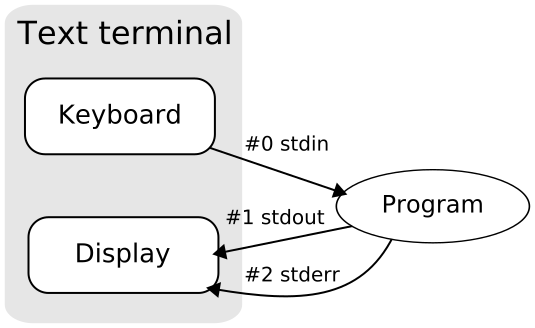
\includegraphics[width=0.9\columnwidth]{svg/Stdstreams-notitle}
% 		\end{figure}
% 	\end{column}
% 	\begin{column}{0.5\textwidth}
% 		\begin{itemize}
% 			\item stdout
% 			\item stderr
% 			\item stdin
% 		\end{itemize}
% 	\end{column}
% 	\end{columns}
% \end{frame}

% \begin{frame}[fragile] % Verbatim을 썼으므로 fragile표시를 해줘야 함.
% 	\frametitle{코드를 넣은 슬라이드}
% 	다음은 Hello World! 프로그램이다.
% 	c/pyg.sh hello.c 를 하면 나오는 내용을 여기 붙이면 되는 것임.
% \begin{Verbatim}[commandchars=\\\{\}]
% \PY{c+cp}{#}\PY{c+cp}{include <stdio.h>}

% \PY{k+kt}{int} \PY{n+nf}{main}\PY{p}{(}\PY{p}{)}
% \PY{p}{\PYZob{}}
%         \PY{n}{fprintf}\PY{p}{(} \PY{n}{stderr}\PY{p}{,} \PY{l+s}{"}\PY{l+s}{Program terminated with error!}\PY{l+s+se}{\PYZbs{}n}\PY{l+s}{"} \PY{p}{)}\PY{p}{;}
%         \PY{k}{return} \PY{l+m+mi}{1}\PY{p}{;}
% \PY{p}{\PYZcb{}}
% \end{Verbatim}
% \end{frame}

% \subsection{서브섹션을 가르면 진도표에 반영됨}

% \begin{frame}
% 	\frametitle{Caeser Cypher II}
% 	{\em \Large Practice1 - Caeser Cypher II}

% 	\vspace{5mm}
% 	중간 타이틀로서 나름 깔끔한듯.
% 	part기능에는 좀 어울리지 않아서 손으로 직접... 읔;;
% \end{frame}

% \section{다른 섹션}

% \begin{frame}[containsverbatim]
% 	\frametitle{그냥 verbatim}
% 	터미널의 출력 따위
% 	\begin{verbatim}
% 	$ chmod -x a.out
% 	$ chmod +x a.out
% 	$ chmod -r test.c
% 	$ chmod +r test.c
% 	$ chmod -w test.c
% 	$ chmod +w test.c
% 	\end{verbatim}
% \end{frame}

% \subsection{Practice2 - chmod}

% \begin{frame}
% 	\frametitle{Practice2 - chmod}
% 	{\em \Large Practice2 - chmod}

% 	\vspace{5mm}
% 	set, unset, get 함수를 완성하여 chmod를 따라해보자.
% 	set, unset, get함수에는 if문이 필요 없다.
% \end{frame}

